\documentclass[a4paper,11pt]{scrartcl}
\usepackage{fullpage}
\usepackage[utf8]{inputenc}
\usepackage[english]{babel}
\usepackage{amssymb}
\usepackage{amsmath}
\usepackage{amsthm}
\usepackage{listings}
\usepackage{graphicx}
\usepackage{cite}

\usepackage[usenames,dvipsnames]{pstricks}
\usepackage{epsfig}
\usepackage{pst-grad} % For gradients
\usepackage{pst-plot} % For axes

\title{Seminararbeit Numerik}
\subtitle{Iterative Solvers - Algebraic Multigrid}
\author{Bernd Schwarzenbacher, Daniel Herold}

\begin{document}
\maketitle
\tableofcontents
\pagebreak

\section{Motivation}
To solve big systems of linear equations the conjugate gradient method is the
most used iterative method. For faster convergence speed the condition of the
problem is further improved with a so-called preconditioner.
The original problem is therefore substituted by the preconditioned problem:
$$b-Ax = 0 \iff x + \tau C^{-1} (b-Ax) = x$$
Where the matrix $C$ denotes the preconditioner.

The Algebraic Multigrid (AMG) method combines several bad preconditioners to
obtain a good preconditioner in total. It belongs to the family of general
Multigrid (MG) methods which recursively coarsen the original matrix and
project the problem on this coarser spaces by use of a prolongation matrix.
On the coarser levels, low frequency errors in the solution are corrected
faster. The AMG method uses only the information in the system matrix to
compute the coarsening and further the projection matrix. It does so by
weighting the relative strength of connecting vertices to determine which
vertices should collapse on the next level.
\cite{numerik} \cite{numpde}

In the application of the AMG preconditioner we use one forward and one
backward Gauß-Seidel preconditioner per level. Additionally a
transposed matrix vector multiplication is needed to project onto the
coarse space. See Listing~\ref{lst:mult} for more details on the algorithm.
Those three points are subject to performance improvements by parallelization.

\section{Sparsematrices}
Most matrices are stored in the Compressed Column Storage (CCS) format.
The commands {\em firsti[k]} and {\em lasti[k]} provide the position of the
first and last entry of the row k in the indexvector. One
iteration through one row ist very easy to provide.

\lstset{language=C++, numbers=none, captionpos=b,
        caption={Row-iteration of sparsematrices }}
\begin{lstlisting}
for (int j = firsti[k]; j < lasti[k]; ++j)
      {...}

\end{lstlisting}

The difficulty with sparsematrices is the iteration among any other order as
the next section will show.

\section{Matrix vector multiplication}

The multiplication of a sparsematrix and a given vector is very simple.
The entry k of the outcoming vector is given by the summation of the products
of the matrixentries in the row k with the entries of the vector. In other
words one entry of the outcoming vector depends only on one row of the matrix
and vice versa.

One of the difficulties of parallelization is given by multiple writing
performances on a single variable at the same time. In the case of a simple
 matrix vector multiplication this is no big deal to handle: Each row has to be
executed by a single task, there is no limitation in which order which task
 calculates 'his' vectorentry.

\lstset{language=C++, numbers=left, captionpos=b,
        caption={Matrix vector multiplication with parallel for section}}
\begin{lstlisting}
void MultAddParallel (double s, const BaseVector & x, BaseVector & y) const  {

#pragma omp parallel for
    for (int i = 0; i < this->Height(); ++i)
    {
      int first = firsti [i];
      int last  = firsti [i+1];

      for (int j = first; j < last; ++j)
      {
        y(i) += s * data[j] * x(colnr[j]);
      }
    }
  }

\end{lstlisting}

\subsection{Transposed matrix vector multiplication}

To provide the multiplication of the transposed of a matrix and a given vector
 a sequential script is written in a similar way.

\lstset{language=C++, numbers=none, captionpos=b,
        caption={Transposed vector multiplication}}
\begin{lstlisting}
...
    for (int i = 0; i < this->Height(); ++i)
    {
      int first = firsti [i];
      int last  = firsti [i+1];

      for (int j = first; j < last; ++j)
      {
        y(colnr[j]) += s * data[j] * x(i);
      }
    }
...
\end{lstlisting}

The difference is the dependency of a single outcoming entry. It is calculated
 by the entries of a column of the matrix - but because of the storage it is not
possible to iterate through one column in an efficient way. The iteration through 
rows is no problem for the sequential code, but parallelization causes some
problems.

 If the algorithm has to iterate through one row of the matrix, simple 
parallelization would probably cause issues in some outcoming entries
 due to multiple writing performances at the same time. In particular it would
possible that one task which iterates through the first rows of the matrix
writes at one entry of the outcoming vector at the same time as another one
does, which iterates through the lower part of the matrix.

Reading and writing processes for the same variable at nearly the same 
time can cause wrong values as shown in figure \ref{figure:parallelwriting}. Two
tasks are trying to write at the same variable at nearly the same time. The second
starts his procedure before task 1 has finished and overwrites the result of it.

\begin{figure}[ht]
\label{figure:parallelwriting}
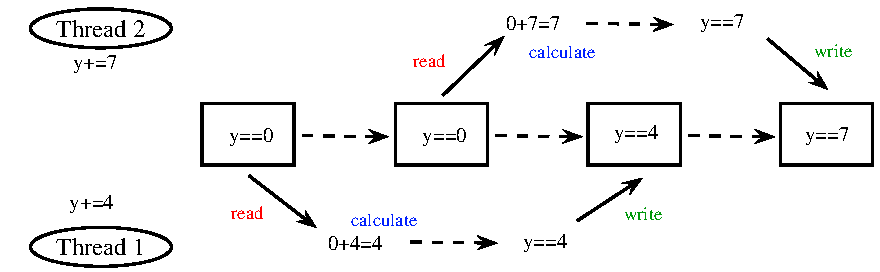
\includegraphics{graphic/parallel_writing_problem.pdf}
\caption{Problem with Parallelization of Writing Processes}
\end{figure}

Some ideas to solve this problem are:

\begin{itemize}

\item atomic writing process (easy to program, but very inefficient)
\item atomic writing process with dynamic task partioning
\item atomic writing process with static thread seperation
\item matrix coloring without any atomic processes

\end{itemize}

All of this solutions efficiencies depend on the number of entries in the matrix.
Less entries and a larger matrix result in a higher amount of calculations per
 time where a sequential solving of a matrix with a lot of nonzeroelements is
 faster than a parallel solution.

The \textbf{atomic} version is very straight forward. The idea is to avoid the problem
 shown in figure \ref{figure:parallelwriting} by making it atomic. This means
 that only one task is allowed to pass the section at the same time.

\lstset{language=C++, numbers=none, captionpos=b,
        caption={Transposed vector multiplication, atomic section}}
\begin{lstlisting}
...
#pragma omp atomic
          fy(colnr[j]) += s * data[j] * fx(i);
...
\end{lstlisting}

This part is also the bottleneck of this algorithm, because every task has to pass this
line and they lock each other.

The \textbf{dynamic task partitioning} solves another problem of this code. {\em OMP for}
(as used in the atomic version)
 splits the for-loop into a  static amount of iterations for each task. Due to the amount
 of calculations each task has to perform, some will be finished while others
are still working. This relates to the specific structur of the matrix. The
 number of nonzeroelements in each row can be very different in AMG.

Instead it is possible to split the jobs dynamically. Tasks with less work to do will
get another part of the calculation while others still do their first part.

The time that is used for the dynamic assignment can be retrieved by the fair
partitioning of the tasks. The number 100 demands, that not every single loop
 will be assigned dynamically but every 100 of them.

\lstset{language=C++, numbers=none, captionpos=b,
        caption={Dynamic for loop}}
\begin{lstlisting}
...
#pragma omp for schedule (dynamic, 100)
...
\end{lstlisting}

The \textbf{balancing option} performs this action in a similar way, but not 
during thefor-loop itself but at first. The time for the calculation of each line
depends (as mentioned) on the number of nonzeroelements in this row. With a
simple algorithm it is possible to  determine this number for each row of the
 matrix and split the loop due to this partitioning.

\lstset{language=C++, numbers=left, captionpos=b,
        caption={Transposed vector multiplication, static balancing}}
\begin{lstlisting}
void TranMultBalance (double s, const BaseVector & x, BaseVector & y) const
  {
    FlatVector<double> fx = x.FV<double> ();
    FlatVector<double> fy = y.FV<double> ();

    int height = this->Height();

    Array<int> thread_seperation;
#pragma omp parallel //shared(thread_seperation)
    {
      int num_threads = omp_get_num_threads();

#pragma omp single
      {
        thread_seperation = Array<int>(num_threads+1);
        int seperation_step = ceil(this->nze / num_threads);

        int thread_i = 1;
        for (int row = 0; row < height; ++row)
        {
          if (firsti[row] >= thread_i * seperation_step)
          {
            thread_seperation[thread_i] = row;
            ++thread_i;
          }
        }
        thread_seperation[0] = 0;
        thread_seperation[num_threads] = height;
      }

#pragma omp for
      for (int thread_i = 1; thread_i <= num_threads; ++thread_i)
      {
        for (int i = thread_seperation[thread_i-1];
             i < thread_seperation[thread_i]; ++i)
        {
          int first = firsti [i];
          int last  = firsti [i+1];

          for (int j = first; j < last; ++j)
          {
#pragma omp atomic
            fy(colnr[j]) += s * data[j] * fx(i);
          }
        }
      }
    }
  }

\end{lstlisting}

Every method still has the same problem with the atomic operation in its
essential part. To avoid this, we have to make sure that multiple tasks do not
write on the same entry of the outcoming vector at the same time.

To solve this,
 we will "\textbf{color}" each row of the matrix. A group of rows will get the same
color, if they do not write on the same entries. Parallelization of this group
will not cause the problem in figure \ref{figure:parallelwriting}.

Not writing at the same entry is equivalent to not having
any columns with nonzeroelements in common. If we have "the coloring of
the matrix" we
 can iterate through the different colors sequential but parallelize every 
loop through a group of same-colored-rows, because they will not interfere.

Figure \ref{figure:coloring} gives an dempnstrative example of the coloring process.

\begin{figure}[ht]\label{figure:coloring}
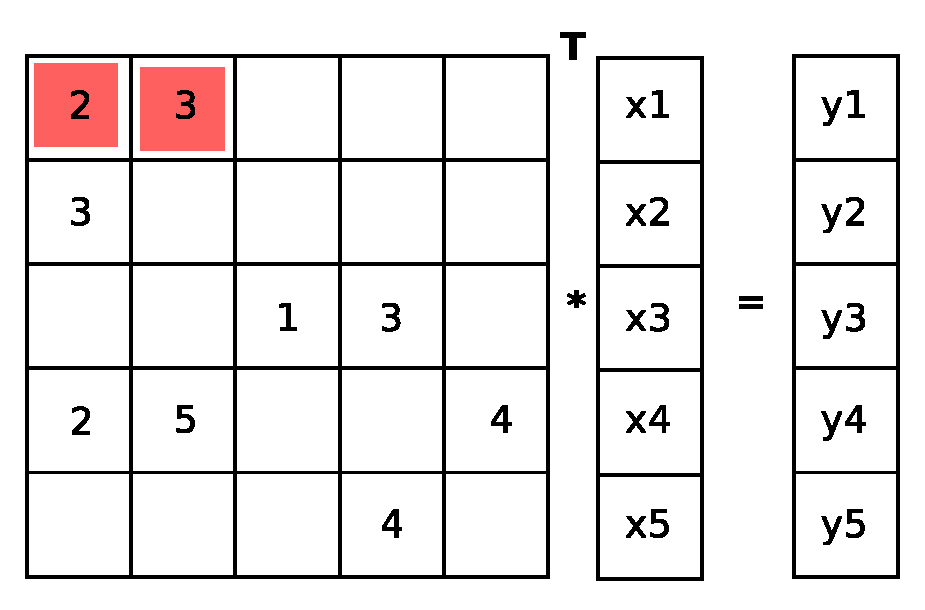
\includegraphics[width=0.32\textwidth]{graphic/coloringT2.eps}\hfill\vline\hfill
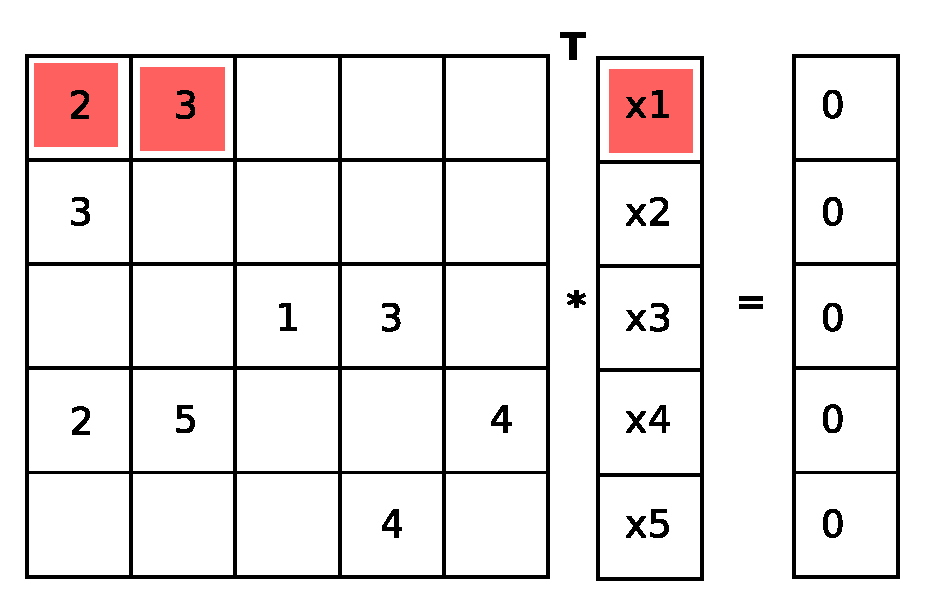
\includegraphics[width=0.32\textwidth]{graphic/coloringT3.eps}\hfill\vline\hfill
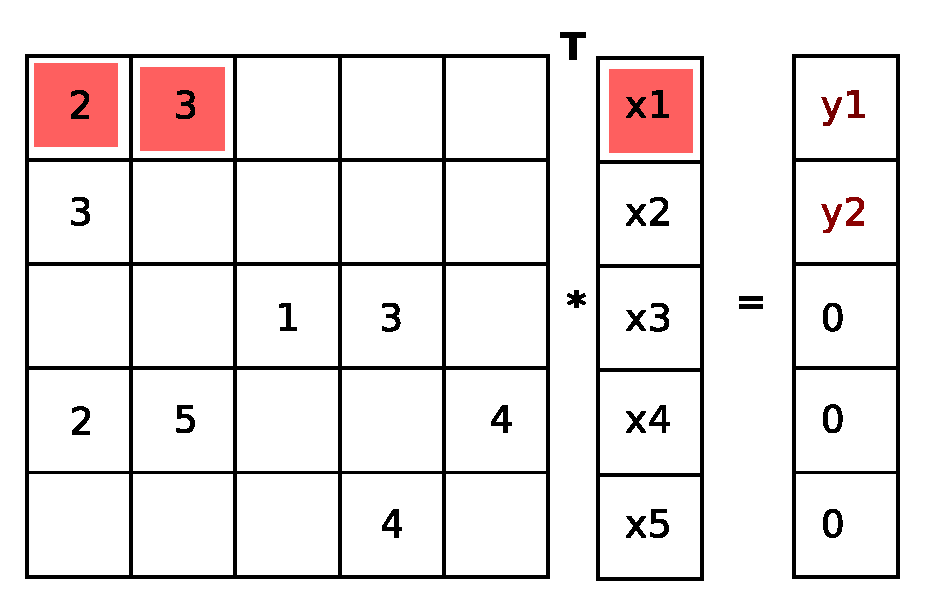
\includegraphics[width=0.32\textwidth]{graphic/coloringT4.eps}
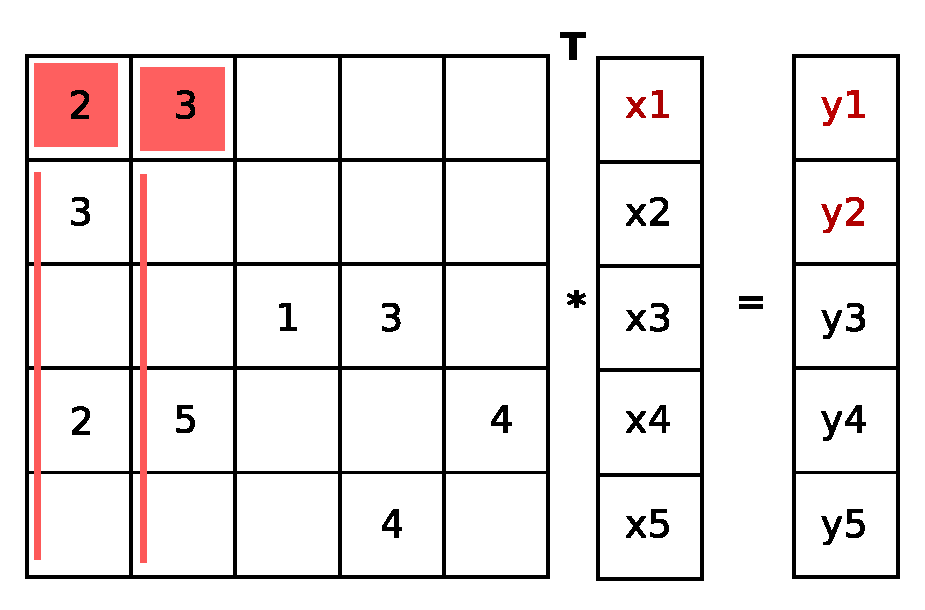
\includegraphics[width=0.32\textwidth]{graphic/coloringT5.eps}\hfill\vline\hfill
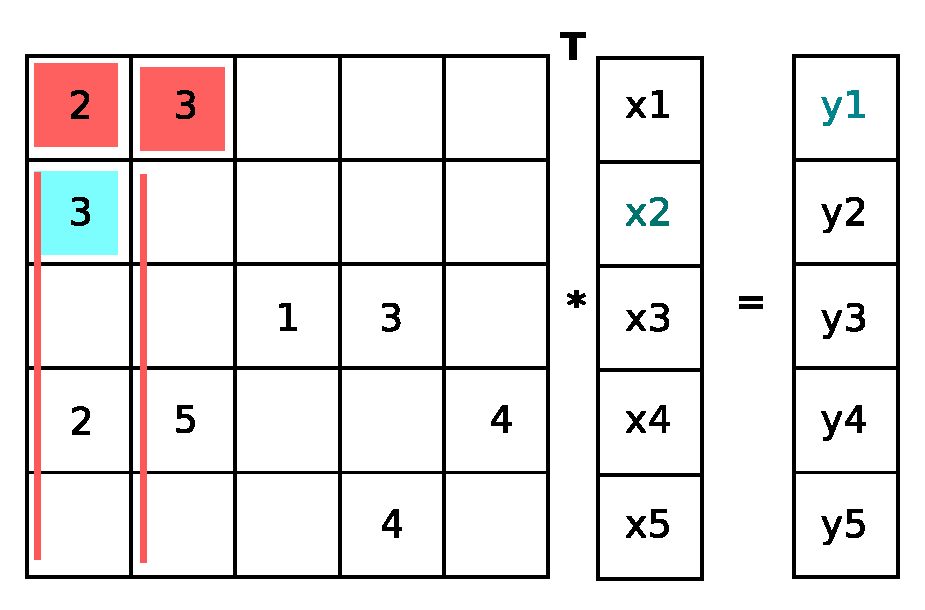
\includegraphics[width=0.32\textwidth]{graphic/coloringT6.eps}\hfill\vline\hfill
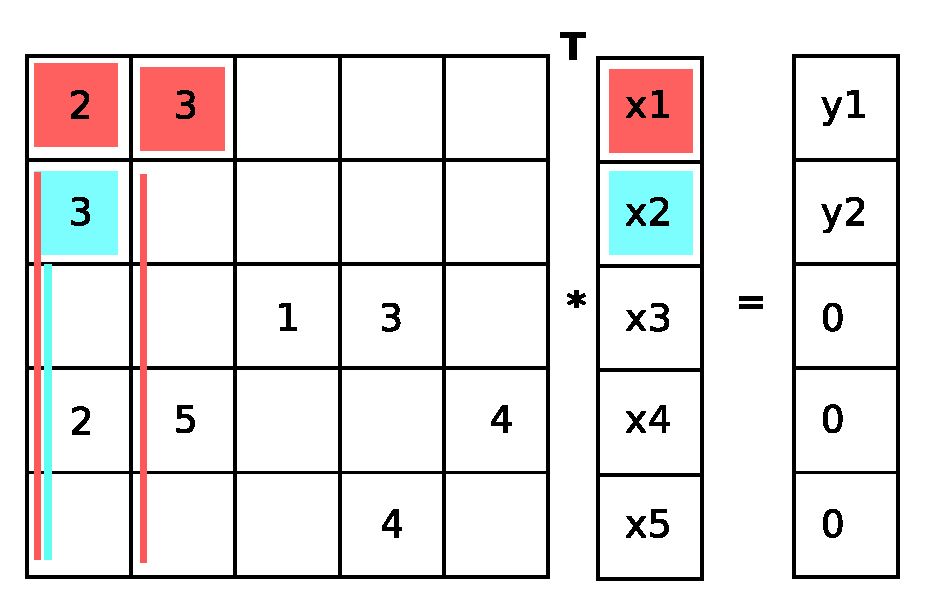
\includegraphics[width=0.32\textwidth]{graphic/coloringT7.eps}
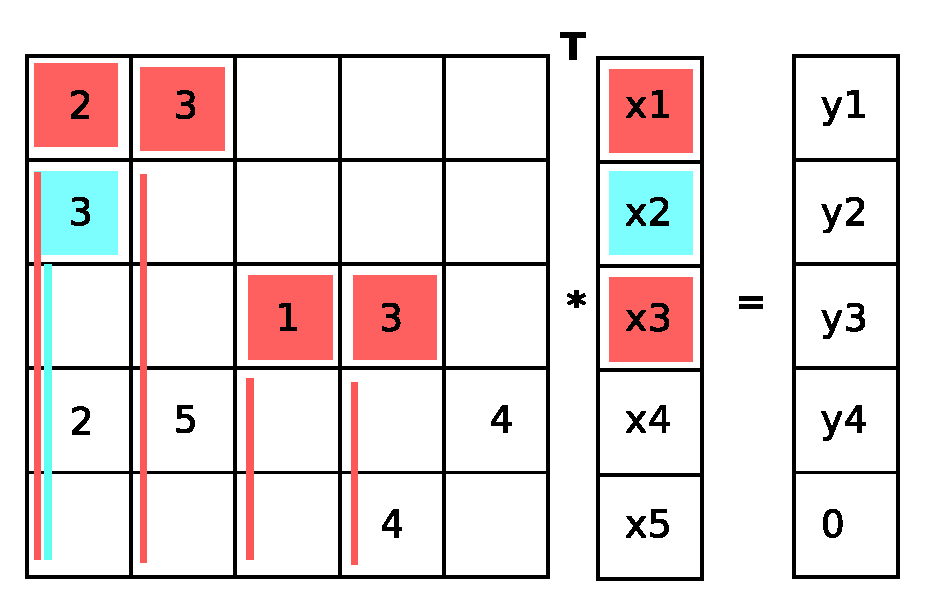
\includegraphics[width=0.32\textwidth]{graphic/coloringT8.eps}\hfill\vline\hfill
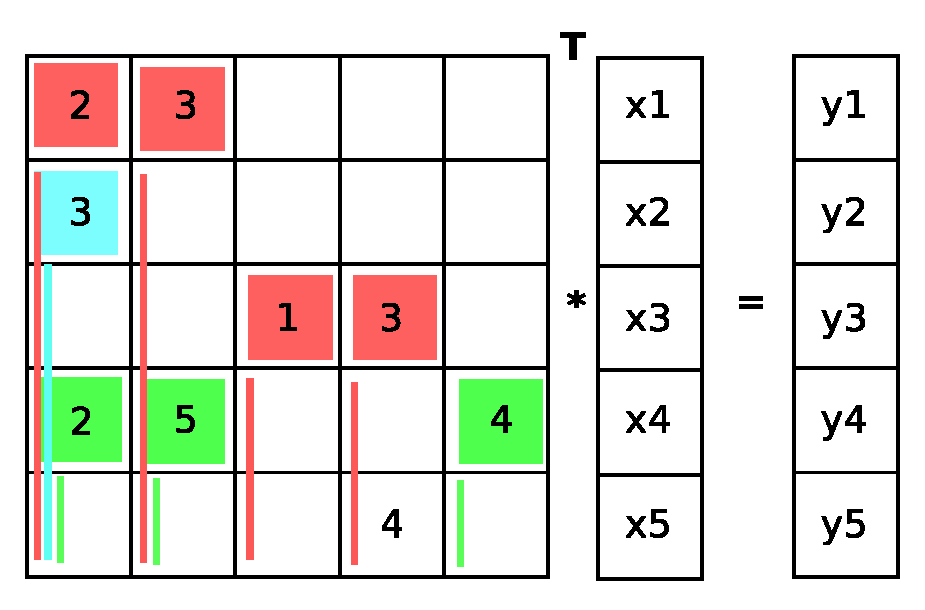
\includegraphics[width=0.32\textwidth]{graphic/coloringT9.eps}\hfill\vline\hfill
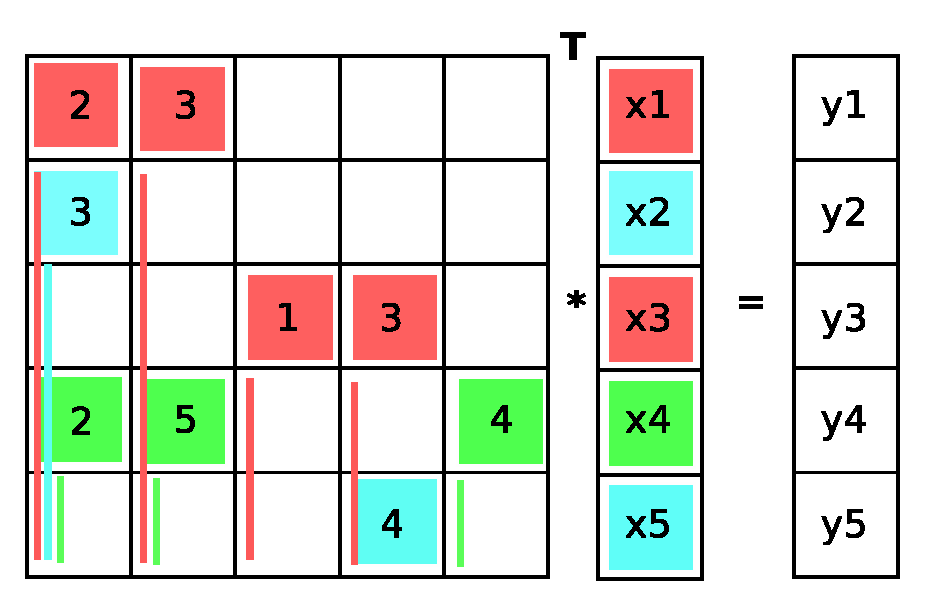
\includegraphics[width=0.32\textwidth]{graphic/coloringT10.eps}
\caption{Coloring of a Simple Matrix}
\end{figure}

This is easy to perform for small matrices. For larger ones we iterate through 
the matrix for every color and store the position of nonzeroelements for the
specific color in a separate mask. Every new row can be compared to the
mask and if all nonzeroentries of the row do not interfere with the mask
it will be colored and the mask updated. As long as there are uncolored
rows of the matrix new colors will be used.

In practice a algorithm is used, which iterates through the matrix for 32 colors
at once. 

\lstset{language=C++, numbers=left, captionpos=b,
        caption={Coloring of a matrix for transposed vector multiplication}}
\begin{lstlisting}
void Coloring ()
  {
    int height = this->Height();
    int width = this->Width();

    Array<int> row_color(height);
    row_color = -1;

    int maxcolor = 0;
    int basecol = 0;

    Array<unsigned int> mask(width);

    int found = 0;

    do
    {
      mask = 0;

      for (int row = 0; row < height; ++row)
      {
        if (row_color[row] >= 0) continue;

        int first = firsti [row];
        int last  = firsti [row+1];

        unsigned check = 0;
        for (int i = first; i < last; ++i)
          check |= mask[colnr[i]];

        if (check != UINT_MAX)
        {
          found++;
          unsigned checkbit = 1;
          int color = basecol;
          while (check & checkbit)
          {
            color++;
            checkbit *= 2;
          }

          row_color[row] = color;
          if (color > maxcolor) maxcolor = color;

          for (int i = first; i < last; ++i)
            mask[colnr[i]] |= checkbit;
        }
      }

      basecol += 8*sizeof(unsigned int); // 32;
    }
    while (found < height);

    Array<int> cntcol(maxcolor+1);
    cntcol = 0;
    for (int row = 0; row < height; ++row)
      ++cntcol[row_color[row]];

    coloring_ = table<int>(cntcol);

    cntcol = 0;
    for (int row = 0; row < height; ++row)
      coloring_[row_color[row]][cntcol[row_color[row]]++] = row;

    std::cout << "needed " << maxcolor+1 << " colors" << std::endl;
  }

\end{lstlisting}

\lstset{language=c++, numbers=left, captionpos=b,
        caption={transposed vector multiplication by coloring a matrix}}
\begin{lstlisting}
void TranMultAdd4 (double s, const BaseVector & x, BaseVector & y)
  {
    FlatVector<double> fx = x.FV<double> ();
    FlatVector<double> fy = y.FV<double> ();

    Coloring();

#pragma omp parallel
    {
      for (auto color : coloring_)
      {
#pragma omp for
        for (int i = 0; i < color.Size(); ++i)
        {
          int first = firsti [color[i]];
          int last  = firsti [color[i]+1];

          for (int j = first; j < last; ++j)
          {
            fy(colnr[j]) += s * data[j] * fx(color[i]);
          }
        }
      }
    }
  }


\end{lstlisting}

\section{Gauß-Seidel-Method}
To solve a linear equation system, we use a special preconditioner, the
Gauß-Seidel-Method. This is similar to the Jacobi-Method, where computing
 the vector $Ax$ is necessary. The difference is,
that we also use the new information optioned by previous computations of
entries of the solution vector. In particular a new entry is given by
$$ x_j^{new} = \frac{1}{A_{jj}} \left(b_{j} - \sum_{k \in K^{new}}A_{jk}
 x_k^{new} - \sum_{k \in K^{old}}A_{jk} x_k^{old}\right)$$
for $j = 1..n$. $K^{new}$ denotes the set of indices of new calculated entries
 of $x$, where $K^{old}$ denotes the old entries.

To perform a parallel algorithm, we have to make sure, that parallel
running tasks do not have to use entries of $x$ which are computed by other
tasks at the same time. The order of computed entries is arbitrary as long as
the method GSSmoothBack is able to compute them in the reverse order.

In the end we implemented a coloring alghorithm.
Similar to the transposed matrix vector multiplication we mark the rows which
can run parallel without influencing them.

\subsection{Coloring}

At calculating the product $A_jx$ which modifies the entry $x_j$ (where $A_j$
denotes the j-th row of the matrix $A$) every entry $x_k$ is used, where
 $A_{jk} \neq 0$. According to this, every row $A_j$, which should be added
to an existing color has to have zeroelements on the positions $A_{jk}$ for
all $k$ indices of current rows of this color.

Instead of testing all remaining rows for this property, we use that $A$ is
 symmetric: $A_{kj} = 0 \Leftrightarrow A_{jk} = 0$. We only have to look
at the specific row we added to one color to determine which rows can also
 relate to it.

The main advance of this method is, that the coloring process has to be
 done only once, whereas it is used by GSSmooth and GSSmoothBack as well.

As in the motivation mentioned, GSSmooth is called with matrices getting
 smaller and GSSmoothBack in reverse order on matrices getting larger.
 The improve of speed is shown in GRAFIK.


\lstset{language=C++, numbers=left, captionpos=b, breaklines=true,
        caption={Multiplication Method of the AMG Preconditioner}}
\begin{lstlisting}
void my_AMG_H1 :: Mult (const ngla::BaseVector & b, ngla::BaseVector & x) const
{
  if (inv) {
    x = (*inv) * b;
    return;
  }

  auto residuum = pmat->CreateVector();
  auto coarse_x = coarsemat->CreateVector();
  auto coarse_residuum = coarsemat->CreateVector();

  x = 0;
  jacobi->GSSmooth (x, b);

  if (recAMG) {
    residuum = b - (*pmat) * x;
    coarse_residuum = ngla::Transpose (*prol) * residuum;

    recAMG->Mult(coarse_residuum, coarse_x);

    x += (*prol) * coarse_x;
  }

  jacobi->GSSmoothBack (x, b);
}
\end{lstlisting}

\label{lst:mult}
\begin{figure}
%% Generated with LaTeXDraw 2.0.8
% Sun Jun 14 10:48:06 CEST 2015
% \usepackage[usenames,dvipsnames]{pstricks}
% \usepackage{epsfig}
% \usepackage{pst-grad} % For gradients
% \usepackage{pst-plot} % For axes
\scalebox{1} % Change this value to rescale the drawing.
{
\begin{pspicture}(0,-2.54)(6.48,2.54)
\definecolor{color641b}{rgb}{0.4823529411764706,0.996078431372549,0.9921568627450981}
\definecolor{color641}{rgb}{0.996078431372549,0.996078431372549,0.996078431372549}
\definecolor{color644b}{rgb}{0.996078431372549,0.37254901960784315,0.37254901960784315}
\definecolor{color651b}{rgb}{0.3058823529411765,1.0,0.3058823529411765}
\definecolor{color661c}{rgb}{0.5019607843137255,0.5019607843137255,0.5019607843137255}
\definecolor{color713}{rgb}{0.9921568627450981,0.34509803921568627,0.34509803921568627}
\definecolor{color715}{rgb}{0.34509803921568627,0.9921568627450981,0.9921568627450981}
\definecolor{color716}{rgb}{0.3568627450980392,0.9921568627450981,0.34509803921568627}
\psframe[linewidth=0.02,linecolor=color641,dimen=outer,fillstyle=solid,fillcolor=color641b](0.83,1.39)(0.07,0.63)
\psframe[linewidth=0.02,linecolor=color641,dimen=outer,fillstyle=solid,fillcolor=color641b](1.85,1.41)(1.09,0.65)
\psframe[linewidth=0.02,linecolor=color641,dimen=outer,fillstyle=solid,fillcolor=color641b](3.89,1.41)(3.13,0.65)
\psframe[linewidth=0.02,linecolor=color641,dimen=outer,fillstyle=solid,fillcolor=color644b](2.89,0.39)(2.13,-0.37)
\psframe[linewidth=0.02,linecolor=color641,dimen=outer,fillstyle=solid,fillcolor=color644b](3.89,0.39)(3.13,-0.37)
\usefont{T1}{ppl}{m}{n}
\rput(3.4664063,-0.03){3}
\psframe[linewidth=0.02,linecolor=color641,dimen=outer,fillstyle=solid,fillcolor=color641b](6.35,1.39)(5.59,0.63)
\psframe[linewidth=0.02,linecolor=color641,dimen=outer,fillstyle=solid,fillcolor=color644b](6.35,0.37)(5.59,-0.39)
\psframe[linewidth=0.02,linecolor=color641,dimen=outer,fillstyle=solid,fillcolor=color651b](1.85,-0.61)(1.09,-1.37)
\psframe[linewidth=0.02,linecolor=color641,dimen=outer,fillstyle=solid,fillcolor=color651b](2.89,-0.63)(2.13,-1.39)
\psframe[linewidth=0.02,linecolor=color641,dimen=outer,fillstyle=solid,fillcolor=color651b](4.91,-0.61)(4.15,-1.37)
\psframe[linewidth=0.02,linecolor=color641,dimen=outer,fillstyle=solid,fillcolor=color651b](6.35,-0.63)(5.59,-1.39)
\psframe[linewidth=0.02,linecolor=color641,dimen=outer,fillstyle=solid,fillcolor=color644b](6.35,-1.63)(5.59,-2.39)
\psframe[linewidth=0.02,linecolor=color641,dimen=outer,fillstyle=solid,fillcolor=color644b](3.89,-1.57)(3.13,-2.33)
\psframe[linewidth=0.02,linecolor=color641,dimen=outer,fillstyle=solid,fillcolor=color644b](6.35,2.37)(5.59,1.61)
\psframe[linewidth=0.02,linecolor=color641,dimen=outer,fillstyle=solid,fillcolor=color644b](0.83,2.43)(0.07,1.67)
\psframe[linewidth=0.02,linecolor=color641,dimen=outer,fillstyle=solid,fillcolor=color644b](1.85,2.39)(1.09,1.63)
\rput(0.0,-2.5){\psgrid[gridwidth=0.028222222,subgridwidth=0.014111111,gridlabels=0.0pt,subgridcolor=color661c](0,0)(0,0)(5,5)}
\usefont{T1}{ppl}{m}{n}
\rput(0.4846875,2.01){2}
\usefont{T1}{ppl}{m}{n}
\rput(1.4964062,2.01){3}
\usefont{T1}{ppl}{m}{n}
\rput(1.515625,0.99){4}
\usefont{T1}{ppl}{m}{n}
\rput(2.4659376,-0.0253125){1}
\usefont{T1}{ppl}{m}{n}
\rput(4.535625,-1.0053124){4}
\usefont{T1}{ppl}{m}{n}
\rput(1.4945313,-1.0053124){5}
\usefont{T1}{ppl}{m}{n}
\rput(3.485625,-2.01){4}
\usefont{T1}{ppl}{m}{n}
\rput(2.4864063,-1.01){3}
\usefont{T1}{ppl}{m}{n}
\rput(0.48640624,0.9853125){3}
\usefont{T1}{ppl}{m}{n}
\rput(3.4645312,0.99){5}
\rput(5.48,-2.5){\psgrid[gridwidth=0.028222222,subgridwidth=0.014111111,gridlabels=0.0pt,subgridcolor=color661c](0,0)(0,0)(1,5)}
\usefont{T1}{ppl}{m}{n}
\rput(5.9428124,2.0146875){x1}
\usefont{T1}{ppl}{m}{n}
\rput(5.9414062,0.9853125){x2}
\usefont{T1}{ppl}{m}{n}
\rput(5.945,-0.03){x3}
\usefont{T1}{ppl}{m}{n}
\rput(5.9492188,-1.0053124){x4}
\usefont{T1}{ppl}{m}{n}
\rput(5.943594,-2.01){x5}
\psline[linewidth=0.06cm,linecolor=color713](0.1,1.32)(0.1,-2.36)
\psline[linewidth=0.06cm,linecolor=color713](2.12,-0.62)(2.12,-2.36)
\psline[linewidth=0.06cm,linecolor=color715](1.12,0.38)(1.12,-2.36)
\psline[linewidth=0.06cm,linecolor=color716](3.1,-1.56)(3.1,-2.38)
\end{pspicture} 
}



\end{figure}

\lstset{language=c++, numbers=left, captionpos=b,
        caption={Gauß-Seidel coloring and balancing}}
\begin{lstlisting}

  void JacobiPrecond<TM,TV_ROW,TV_COL> :: Coloring ()
  {
    //static Timer timer("JacobiPrecond::Coloring");
    //RegionTimer reg (timer);

    int height = mat.Height();
    int width = mat.Width();

    Array<int> row_color(height);
    row_color = -1;

    int maxcolor = 0;
    int basecol = 0;

    Array<unsigned int> mask(width);

    int found = 0;

    int num_threads = task_manager->GetNumThreads();

    do
    {
      mask = 0;

      int block_size = ceil((double)height / (double)num_threads);

      for (int block_row = 0; block_row < block_size; ++block_row)
      {
        for (int threadi = 0; threadi < num_threads; ++threadi)
        {
          int row = block_row + threadi * block_size;
          if (row >= height) break;
          if (row_color[row] >= 0) continue;

          int first = mat.firsti [row];
          int last  = mat.firsti [row+1];

          unsigned check = 0;
          for (int i = first; i < last; ++i)
            check |= mask[mat.colnr[i]];

          if (check != UINT_MAX) // 0xFFFFFFFF)
          {
            found++;
            unsigned checkbit = 1;
            int color = basecol;
            while (check & checkbit)
            {
              color++;
              checkbit *= 2;
            }

            row_color[row] = color;
            if (color > maxcolor) maxcolor = color;

            mask[row] |= checkbit;
          }
        }
      }

      basecol += 8*sizeof(unsigned int); // 32;
    }
    while (found < height);

    Array<int> cntcol(maxcolor+1);
    cntcol = 0;
    for (int row = 0; row < height; ++row)
      ++cntcol[row_color[row]];

    coloring_ = Table<int>(cntcol);

    cntcol = 0;
    for (int row = 0; row < height; ++row)
      coloring_[row_color[row]][cntcol[row_color[row]]++] = row;

    balancing_.SetSize (maxcolor+1);
    for (auto c : Range (balancing_))
    {
      balancing_[c].Calc (coloring_[c].Size(),
        [&] (int bi)
        {
          return 5 + mat.GetRowIndices(coloring_[c][bi]).Size();
        });
    }

    //cout << "Balancing: " << balancing_ << endl;
    std::cout << "needed " << maxcolor+1 << " colors" << std::endl;
  }

\end{lstlisting}

\lstset{language=c++, numbers=left, captionpos=b,
        caption={Gauß-Seidel Smooth}}
\begin{lstlisting}



  void JacobiPrecond<TM,TV_ROW,TV_COL> ::
  GSSmooth (BaseVector & x, const BaseVector & b) const
  {
    //static Timer timer("JacobiPrecond::GSSmooth");
    //timer.AddFlops (mat.NZE());
    //RegionTimer reg (timer);

    FlatVector<TV_ROW> fx = x.FV<TV_ROW> ();
    // dynamic_cast<T_BaseVector<TV_ROW> &> (x).FV();
    const FlatVector<TV_ROW> fb = b.FV<TV_ROW> ();
    // dynamic_cast<const T_BaseVector<TV_ROW> &> (b).FV();

    for (int j = 0; j < this->coloring_.Size(); ++j)
    {
      auto color = this->coloring_[j];
      ParallelFor( this->balancing_[j],
        [this, fx, fb, color] (int i)
        {
          int row = color[i];
          if (!this->inner || this->inner->Test(row))
          {
            TV_ROW ax = mat.RowTimesVector (row, fx);
            fx(row) += invdiag[row] * (fb(row) - ax);
          }
        }, 4);
    }
  }
\end{lstlisting}

\lstset{language=c++, numbers=left, captionpos=b,
        caption={Gauß-Seidel SmoothBack}}
\begin{lstlisting}
  void JacobiPrecond<TM,TV_ROW,TV_COL> ::
  GSSmoothBack (BaseVector & x, const BaseVector & b) const
  {
    //static Timer timer("JacobiPrecond::GSSmoothBack");
    //timer.AddFlops (mat.NZE());
    //RegionTimer reg (timer);

    FlatVector<TV_ROW> fx = x.FV<TV_ROW> ();
    // dynamic_cast<T_BaseVector<TV_ROW> &> (x).FV();
    const FlatVector<TV_ROW> fb = b.FV<TV_ROW> ();
    //dynamic_cast<const T_BaseVector<TV_ROW> &> (b).FV();

    for (int j = this->coloring_.Size()-1; j >= 0; --j)
    {
      auto color = this->coloring_[j];
      ParallelFor( this->balancing_[j],
        [this, fx, fb, color] (int i)
        {
          int row = color[i];
          if (!this->inner || this->inner->Test(row))
          {
            TV_ROW ax = mat.RowTimesVector (row, fx);
            fx(row) += invdiag[row] * (fb(row) - ax);
          }
        }, 4);
    }
  }


\end{lstlisting}

\begin{figure}
    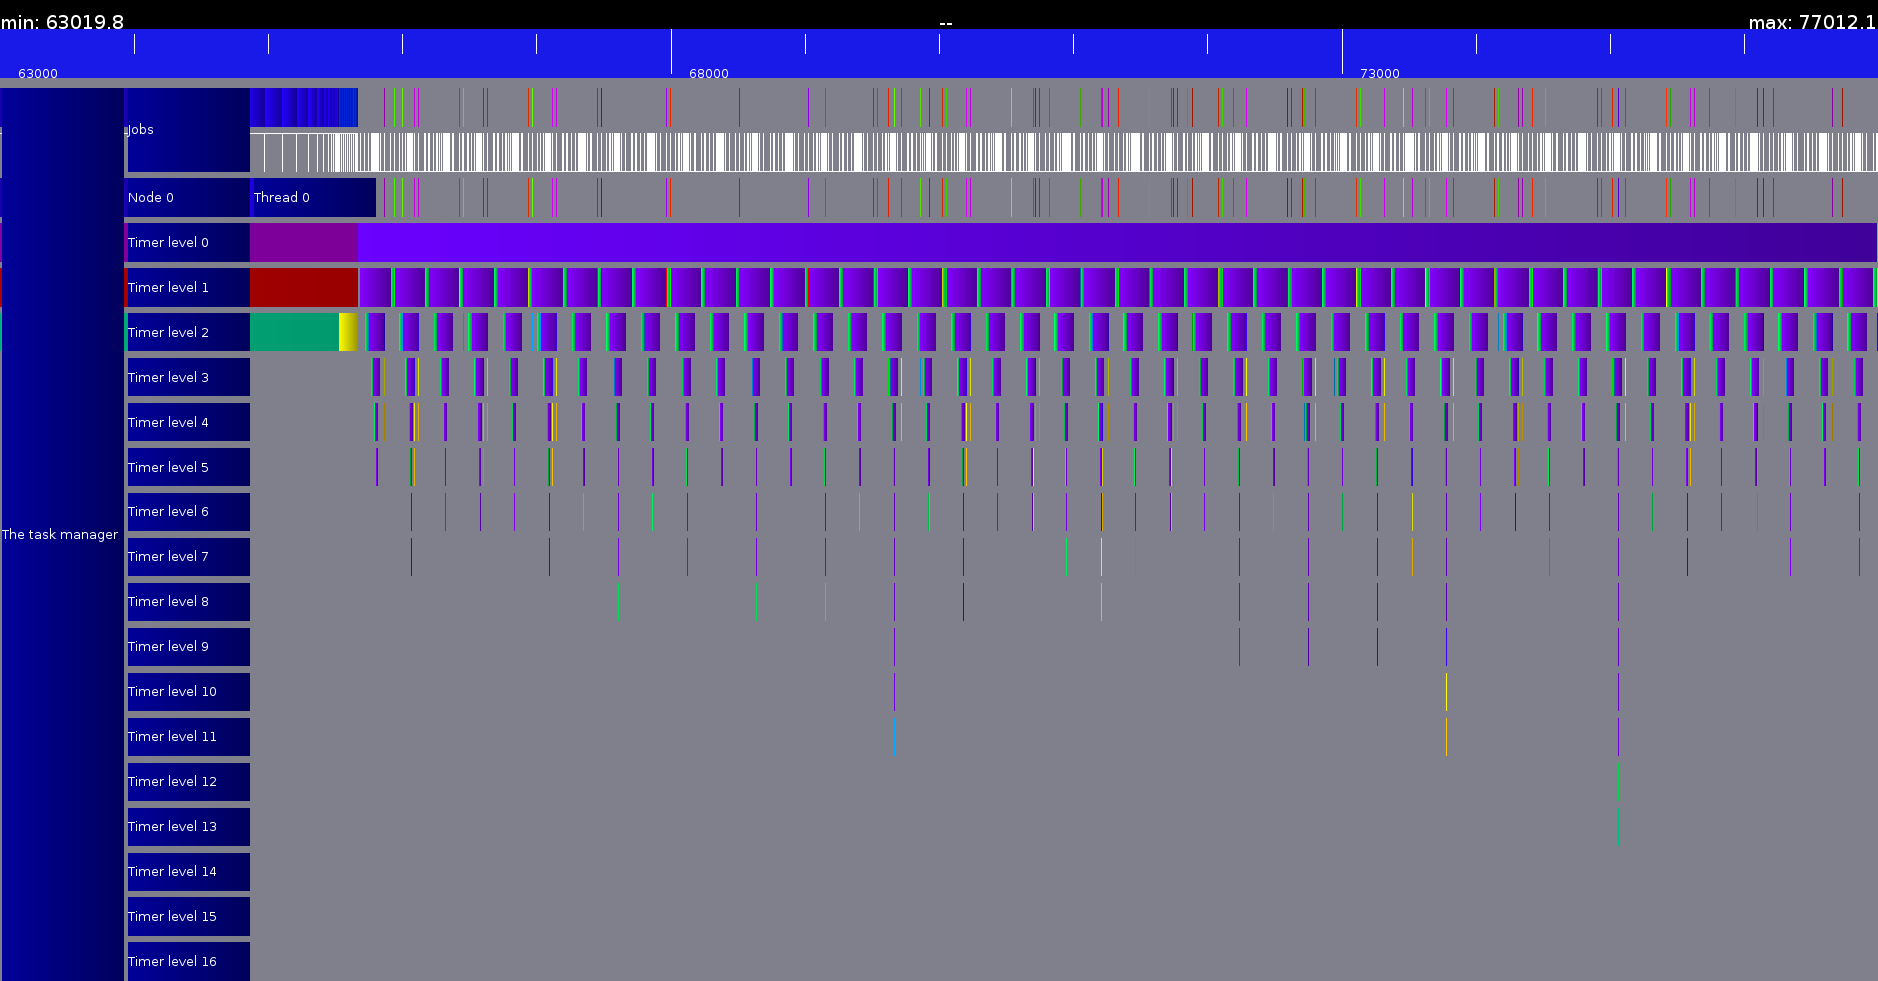
\includegraphics[width=1\textwidth]{seq.png}
    \caption{AMG sequential}
\end{figure}

\begin{figure}
    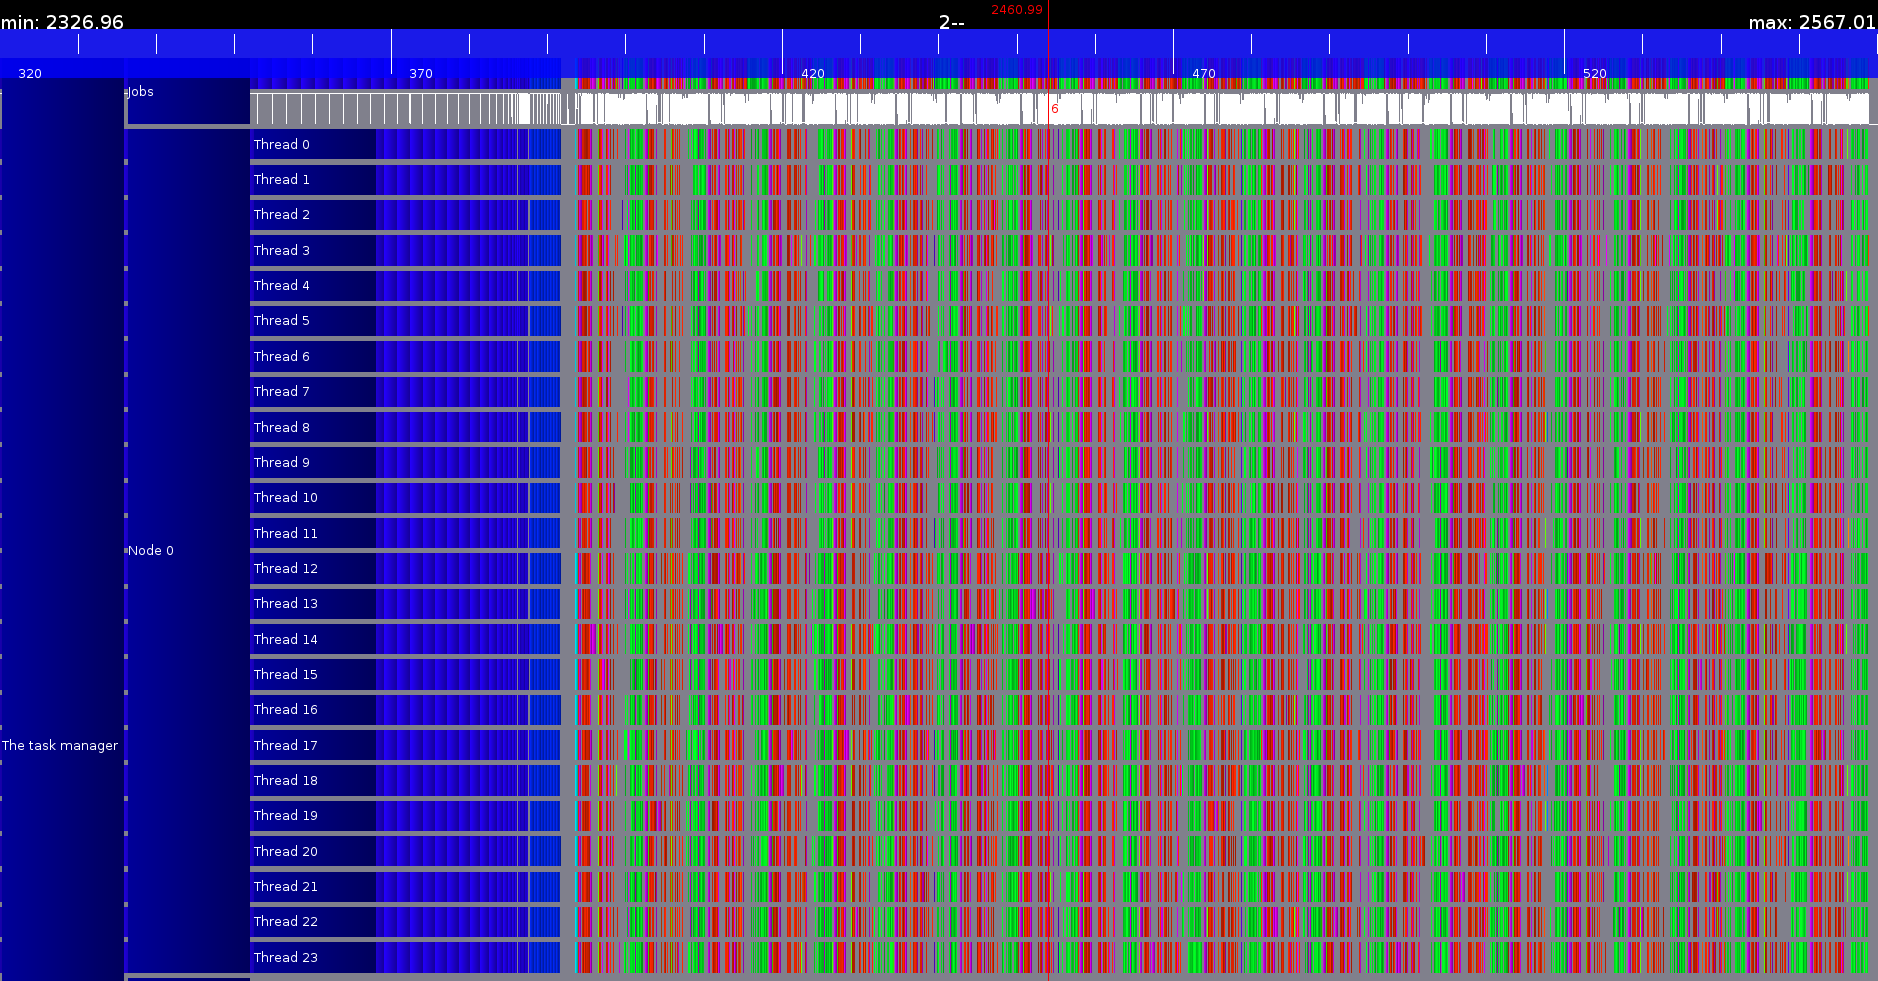
\includegraphics[width=1\textwidth]{iterations_trace.png}
    \caption{AMG parallel}
\end{figure}

\begin{figure}
    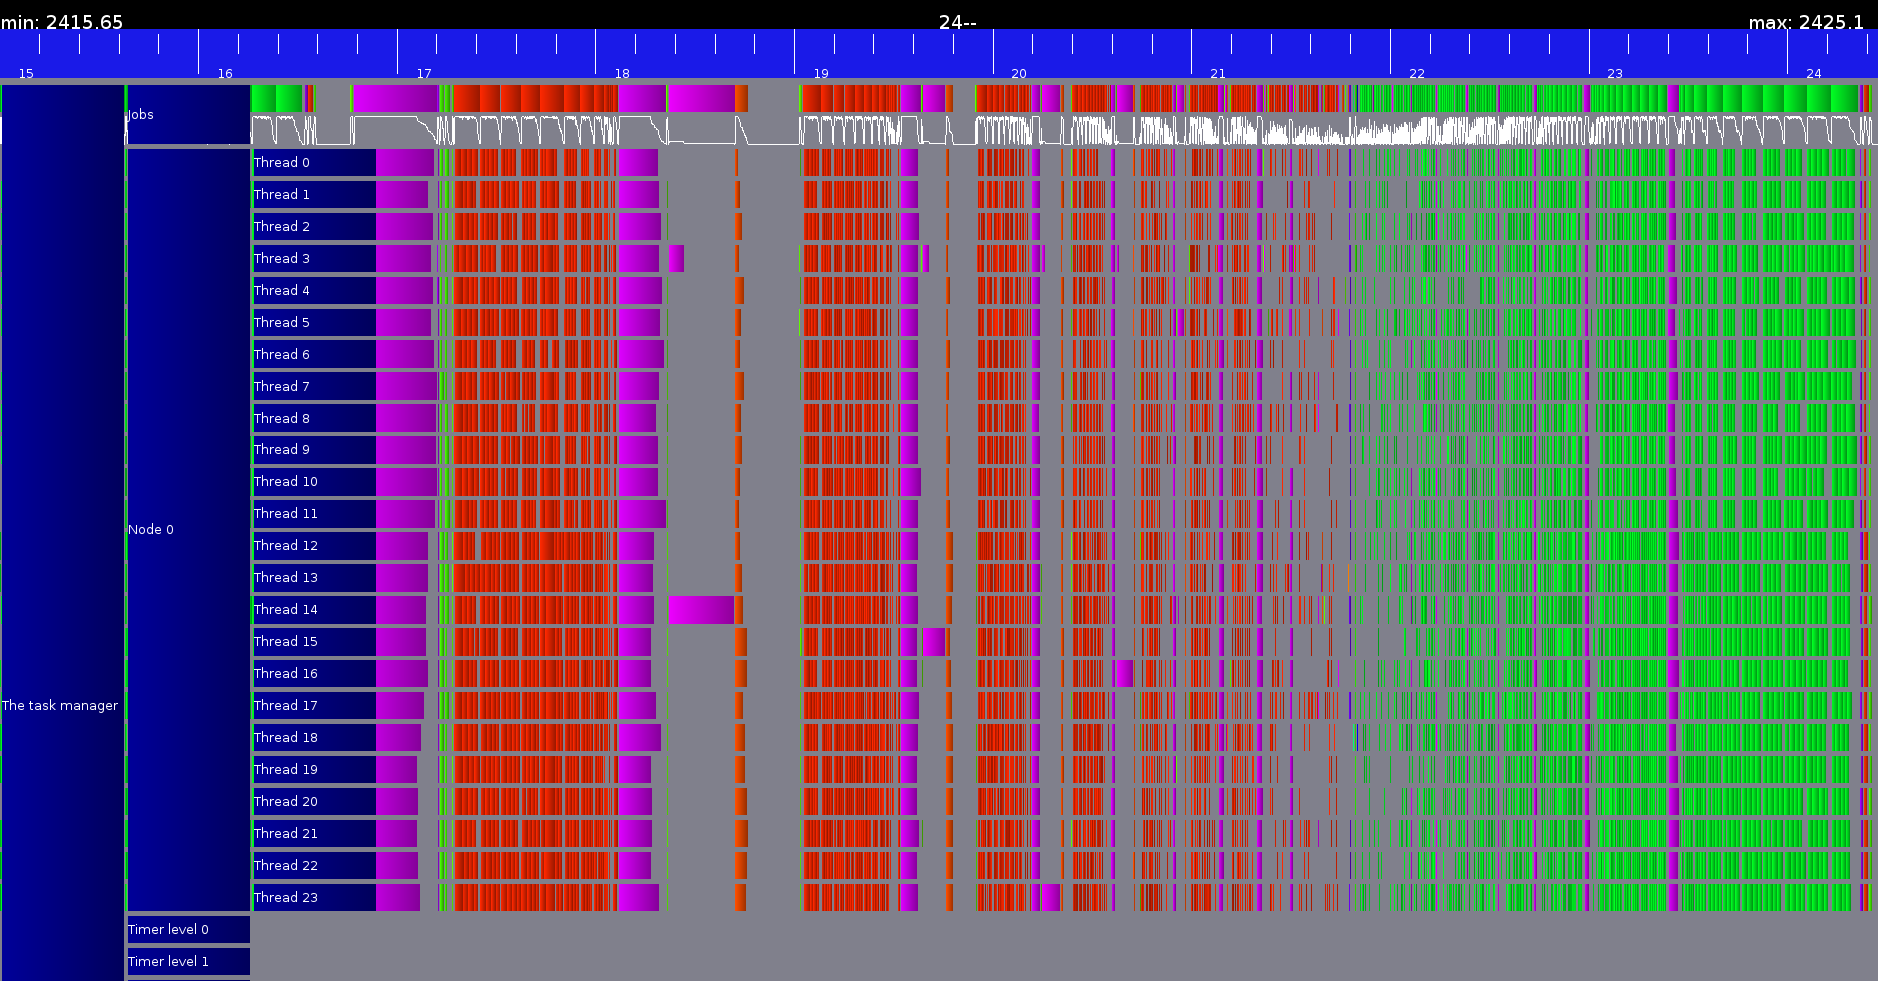
\includegraphics[width=1\textwidth]{one_iteration.png}
    \caption{AMG single parallel recursion}
\end{figure}

\bibliography{doc}{}
\bibliographystyle{plain}
\end{document}
